\documentclass[11pt]{beamer}    % Presentacion
\usepackage[spanish]{babel}     % Español
\usepackage[utf8]{inputenc}     % Aceptar entrada UTF-8
\usepackage{graphicx}           % Insertar imagenes
\usepackage{float}              % Entornos flotantes
\usepackage{pgfgantt}           % Diagrama de Gantt
\usepackage{subcaption}
\usepackage{tikz}
\usepackage{multirow}

% Ajustar tikz
\usetikzlibrary{positioning, arrows, shapes, automata}
\tikzset{Node style/.style={thick, draw=black, circle, align=center, minimum width=70pt}}
\tikzset{
	->, % Hace que los arcos sean dirigidos
	>=stealth, % Hace que la punta de las flechas sean gruesas
	node distance=7cm, % Distancia minima entre nodos
}


\usetheme{metropolis}           % Usar el tema metropolis
\setlength{\unitlength}{1cm}    % Configurar el entorno picture

%%%%%%%%%%%%%%%%%%%%%%%%%%%%%%%%%%%%%%%%%%%%%%%%%%%%%%%%%%%%%%%%%%%%%%%%%%%%%%%%
% Configurar footer
%\setbeamertemplate{frame footer}{\insertshortauthor \quad \quad \insertshortsubtitle}
%\setbeamercolor{footline}{fg=gray}
\setbeamertemplate{section in toc}[sections numbered]
\metroset{numbering=fraction}

%%%%%%%%%%%%%%%%%%%%%%%%%%%%%%%%%%%%%%%%%%%%%%%%%%%%%%%%%%%%%%%%%%%%%%%%%%%%%%%%
% Portada
\title{Desarrollo de una arquitectura reactiva y deliberativa usando
planificación en el entorno de juegos GVGAI}
\subtitle{Trabajo Fin de Grado}
\author[Vladislav Nikolov]{\textbf{Autor} Vladislav Nikolov Vasilev \and
    \textbf{Director} Juan Fernández Olivares
}
\date{\today}
\institute{Departamento de Ciencias de la Computación e Inteligencia Artificial \\
    Escuela Técnica Superior de Ingenierías Informática y de Telecomunicación \\
    Universidad de Granada
}

\begin{document}
    % Insertar pagina de titulo
    \maketitle

    % Insertar indice
    \begin{frame}{Índice}
        \tableofcontents
    \end{frame}

    \section{Introducción}
    \begin{frame}{Motivación}
        \begin{itemize}
            \item Planificación automática como potente herramienta para la resolución de problemas.

            \item Integrada exitosamente en aplicaciones reales pero no en videojuegos.

            \item Videojuegos presentan entornos \alert{dinámicos} y \alert{complejos}.
            No se puede dar una respuesta rápida.

            \item Desarrollo de agentes para juegos concretos cuya componente deliberativa se basa
            en planificación.
        \end{itemize}
    \end{frame}

    \begin{frame}{Objetivo}
        Creación de una arquitectura en el entorno de juegos GVGAI con las siguientes características:

        \begin{enumerate}
            \item Combina componente \alert{reactiva} con \alert{deliberativa} basada en planificación.
            \item Lo suficientemente \textbf{general} para resolver cualquier juego del entorno.
        \end{enumerate}
    \end{frame}

    \begin{frame}{Contribuciones principales}
        \begin{itemize}
            \item Nuevas vías para experimentar con técnicas de planificación en GVGAI.
            \item Herramienta educativa.
        \end{itemize}
    \end{frame}

    %%%%%%%%%%%%%%%%%%%%%%%%%%%%%%%%%%%%%%%%%%%%%%%%%%%%%%%%%%%%%%%%%%%%%%%%%%%%%%%%
    \section{Antecedentes}

    \begin{frame}{Trabajos relacionados}
        Propuesta \alert{novedosa}, aunque se han desarrollado arquitecturas para otros
        juegos en específico.

        \begin{figure}
            \centering
            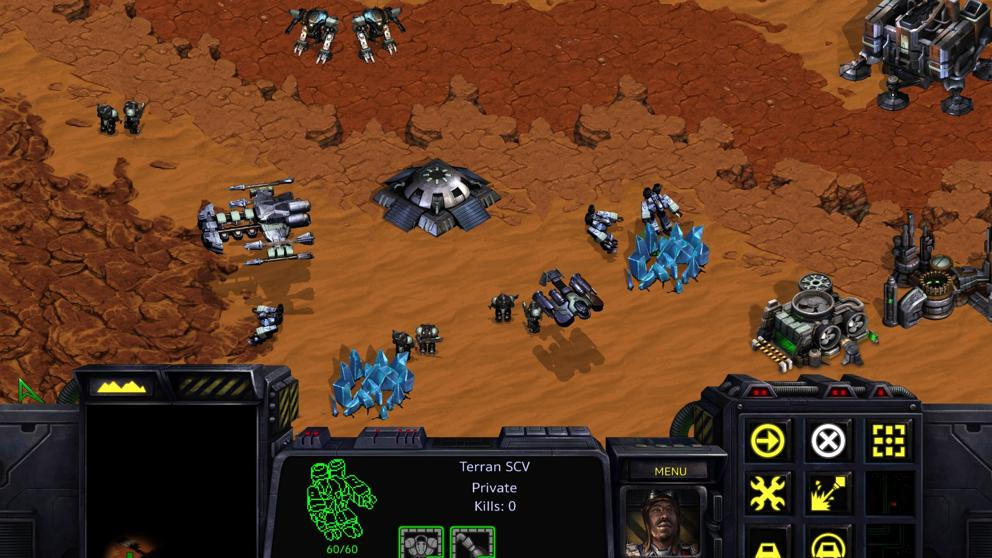
\includegraphics[scale=0.25]{img/presentation/starcraft}
        \end{figure}
    \end{frame}

    \begin{frame}{Planificación}
        \begin{figure}
            \centering
            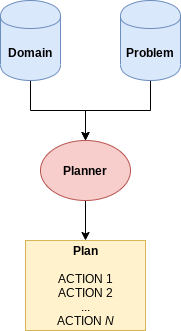
\includegraphics[scale=0.4]{img/presentation/planning}
        \end{figure}
    \end{frame}

    \begin{frame}{PDDL}
        \begin{figure}
            \centering
            \begin{subfigure}[t]{.55\textwidth}
                \centering
                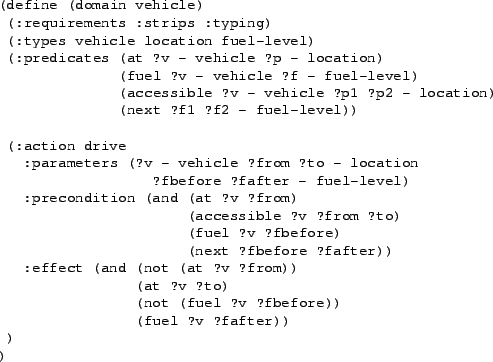
\includegraphics[scale=0.32]{img/presentation/pddl_domain}
                \caption{Dominio de planificación PDDL.}
            \end{subfigure}%
            \begin{subfigure}[t]{.45\textwidth}
                \centering
                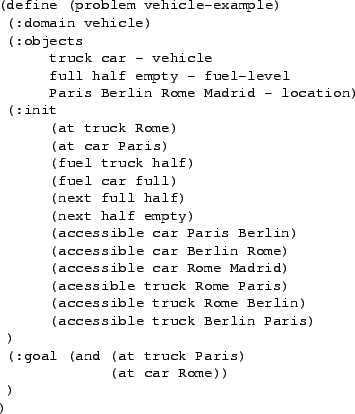
\includegraphics[scale=0.32]{img/presentation/pddl_problem}
                \caption{Problema de planificación PDDL.}
            \end{subfigure}
        \end{figure}
    \end{frame}

    \begin{frame}{Planning.Domains}
        \begin{figure}
            \centering
            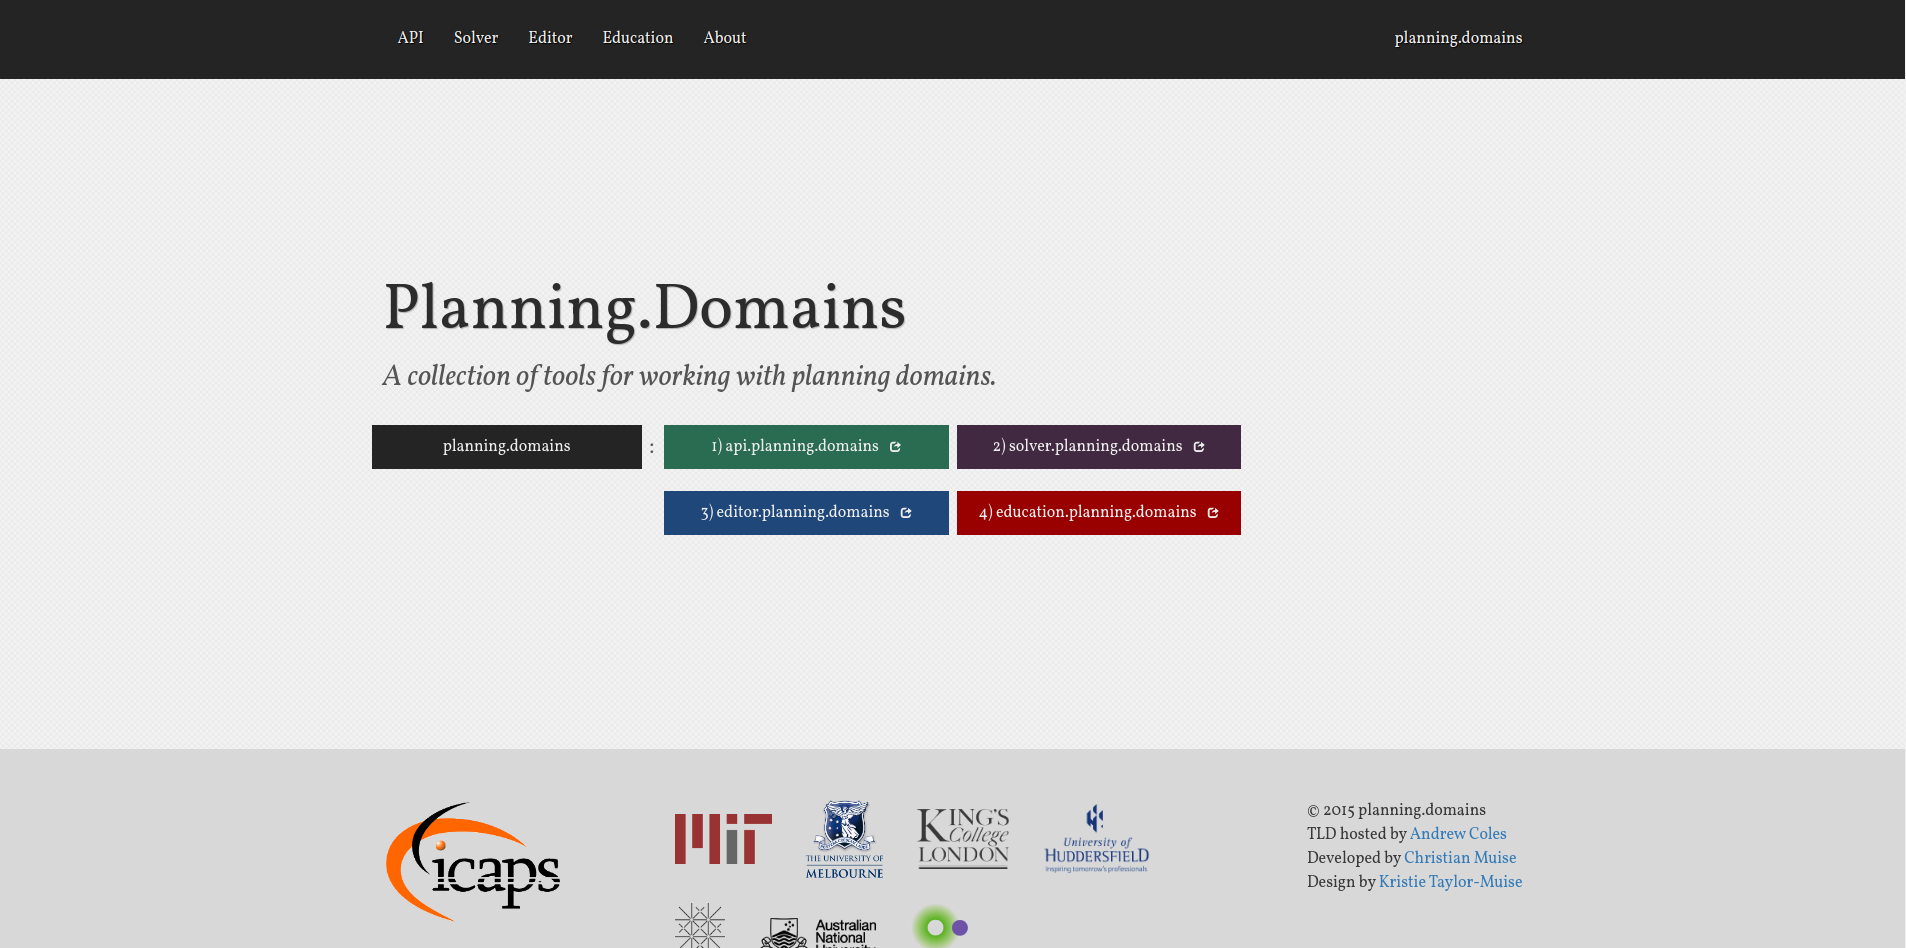
\includegraphics[scale=0.23]{img/presentation/planning-domains}
        \end{figure}
    \end{frame}

    \begin{frame}{GVGAI}
        \begin{figure}
            \centering
            \begin{subfigure}[t]{.5\textwidth}
                \centering
                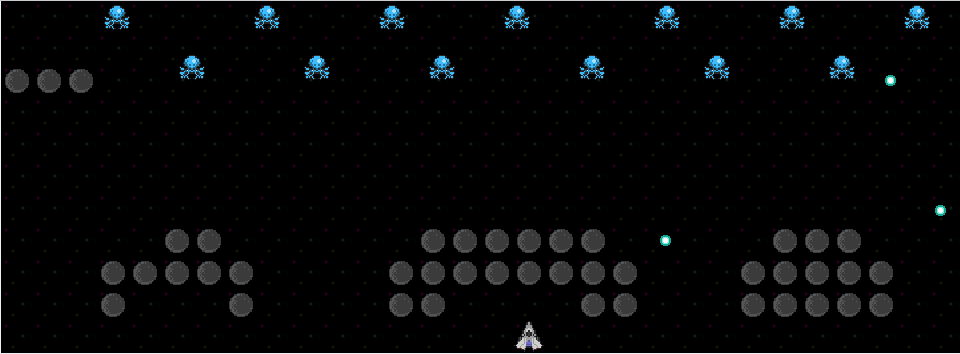
\includegraphics[scale=0.2]{img/presentation/aliens}
            \end{subfigure}%
            \begin{subfigure}[t]{.5\textwidth}
                \centering
                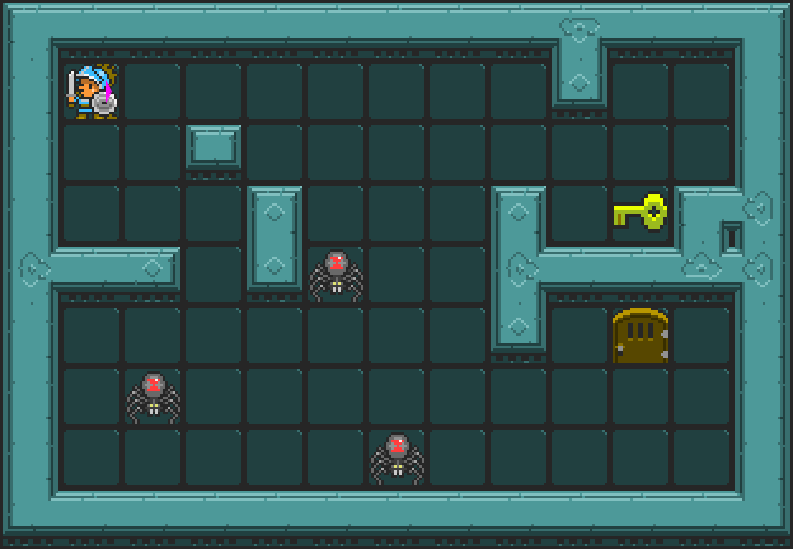
\includegraphics[scale=0.2]{img/presentation/zelda}
            \end{subfigure}
            \par\bigskip
            \begin{subfigure}[t]{.5\textwidth}
                \centering
                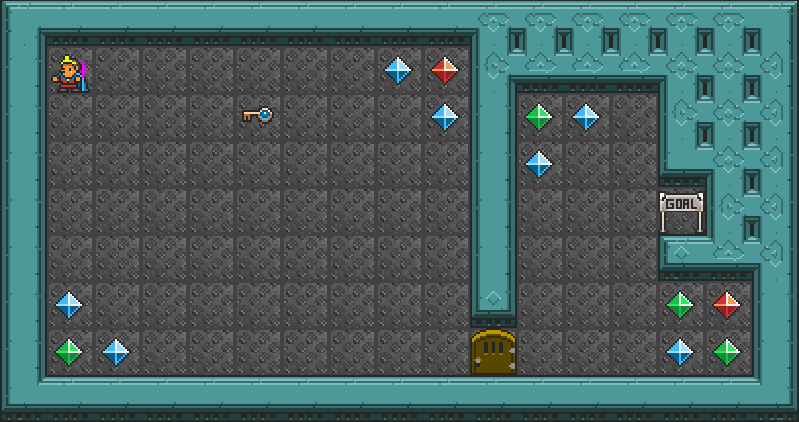
\includegraphics[scale=0.2]{img/presentation/brainman}
            \end{subfigure}%
            \begin{subfigure}[t]{.5\textwidth}
                \centering
                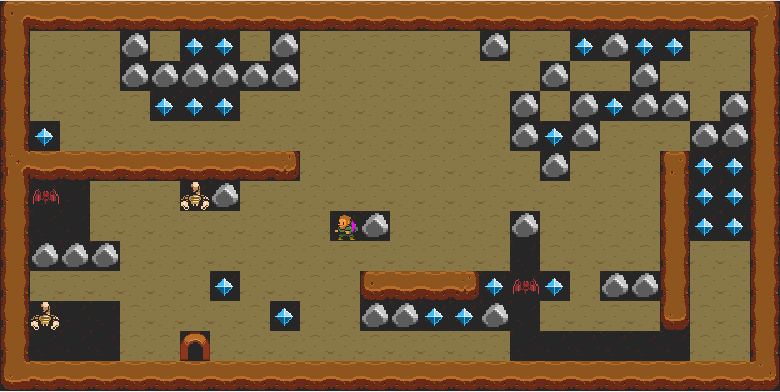
\includegraphics[scale=0.2]{img/presentation/boulderdash}
            \end{subfigure}
        \end{figure}
    \end{frame}

    \begin{frame}{VGDL}
        \begin{figure}
            \centering
            \begin{subfigure}{0.5\textwidth}
                \centering
                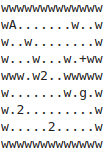
\includegraphics[scale=0.5]{img/presentation/game_lvl}
                \par\bigskip
                {\LARGE$\downarrow{}$}
                \par\bigskip
                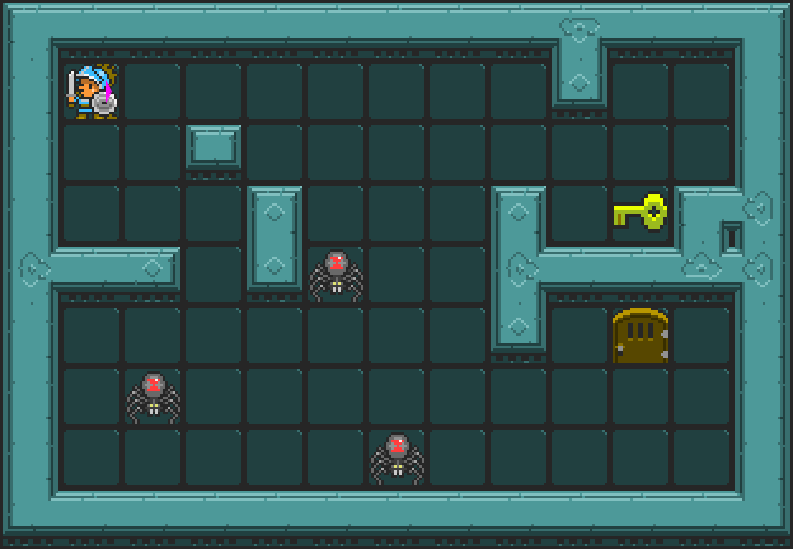
\includegraphics[scale=0.2]{img/presentation/zelda}
            \end{subfigure}%
            \begin{subfigure}{0.5\textwidth}
                \centering
                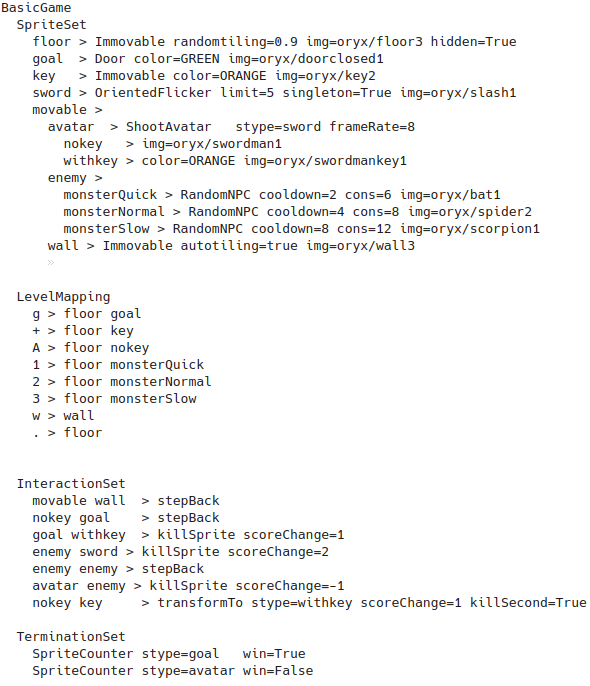
\includegraphics[scale=0.4]{img/presentation/game_def}
            \end{subfigure}
        \end{figure}
    \end{frame}

    %%%%%%%%%%%%%%%%%%%%%%%%%%%%%%%%%%%%%%%%%%%%%%%%%%%%%%%%%%%%%%%%%%%%%%%%%%%%%%%%
    \section{Plan de trabajo}

    \begin{frame}{Metodología}
        \begin{itemize}
            \item Metodología de trabajo basada en \textbf{Scrum}.
            \item Reuniones cada 1-2 semanas:
                \begin{itemize}
                    \item Revisión de objetivos alcanzados
                    \item Resolución de problemas surgidos
                    \item Propuesta de nuevos objetivos
                \end{itemize}
        \end{itemize}
    \end{frame}

    \begin{frame}{Temporización}
        \begin{figure}
            \centering
            \scalebox{0.36}{
                \begin{ganttchart}[%Specs
     y unit title=0.5cm,
     y unit chart=0.7cm,
     vgrid,hgrid,
     title height=1,
     title label font=\bfseries\footnotesize,
     bar/.style={fill=blue},
     bar height=0.4,
     group right shift=0,
     group top shift=0.7,
     group height=.3,
     group peaks width={0.2},
     inline]{1}{36}
    %labels
    \gantttitle{Jul}{3}
    \gantttitle{Ago}{3}
    \gantttitle{Sep}{3}
    \gantttitle{Oct}{3}
    \gantttitle{Nov}{3}
    \gantttitle{Dic}{3}
    \gantttitle{Ene}{3}
    \gantttitle{Feb}{3}
    \gantttitle{Mar}{3}
    \gantttitle{Abr}{3}
    \gantttitle{May}{3}
    \gantttitle{Jun}{3}\\
    % Setting group if any
    \ganttgroup[inline=false]{Estudio}{1}{35}\\
    \ganttbar[inline=false, bar/.style={fill=red}]{Planificación}{1}{4}\\
    \ganttbar[inline=false, bar/.style={fill=red}]{Arquitecturas de planificación}{15}{15}\\
    \ganttbar[inline=false, bar/.style={fill=red}]{Bibliografía complementaria}{34}{35}\\
    
    \ganttgroup[inline=false]{Diseño}{2}{30}\\
    \ganttbar[inline=false, bar/.style={fill=yellow}]{Definición dominio PDDL inicial}{2}{3}\\
    \ganttbar[inline=false, bar/.style={fill=yellow}]{Almacenamiento y gestión de objetivos}{15}{17}
    \ganttbar[inline=false, bar/.style={fill=yellow}]{}{21}{21}\\
    \ganttbar[inline=false, bar/.style={fill=yellow}]{Arquitectura del agente}{21}{22}\\
    \ganttbar[inline=false, bar/.style={fill=yellow}]{Archivo de configuración del sistema}{24}{26}\\
    \ganttbar[inline=false, bar/.style={fill=yellow}]{Definición dominios PDDL nuevos juegos}{27}{28}\\
    \ganttbar[inline=false, bar/.style={fill=yellow}]{Funcionalidad del modo depuración}{29}{30}\\
    
    \ganttgroup[inline=false]{Implementación}{1}{32}\\
    \ganttbar[inline=false, bar/.style={fill=cyan}]{Integración de planificador en GVGAI}{1}{3}\\
    \ganttbar[inline=false, bar/.style={fill=cyan}]{Traducción automática de estados del juego}{5}{12}\\
    \ganttbar[inline=false, bar/.style={fill=cyan}]{Gestión de objetivos}{16}{17}
    \ganttbar[inline=false, bar/.style={fill=cyan}]{}{21}{23}\\
    \ganttbar[inline=false, bar/.style={fill=cyan}]{Control de discrepancias}{21}{23}\\
    \ganttbar[inline=false, bar/.style={fill=cyan}]{Generación automática de archivos de configuración}{26}{27}\\
    \ganttbar[inline=false, bar/.style={fill=cyan}]{Modo depuración}{30}{32}\\
    
    \ganttgroup[inline=false]{Validación}{33}{33}\\
    \ganttbar[inline=false, bar/.style={fill=green}]{Creación de tests}{33}{33}\\
    
    \ganttgroup[inline=false]{Experimentación}{29}{35}\\
    \ganttbar[inline=false, bar/.style={fill=pink}]{Estudio del control de discrepancias}{29}{30}\\
    \ganttbar[inline=false, bar/.style={fill=pink}]{Estudio de la generación de problemas}{35}{35}\\
    
    \ganttgroup[inline=false]{Documentación}{22}{36} \\
    \ganttbar[inline=false, bar/.style={fill=orange}]{Código fuente}{22}{33}\\
    \ganttbar[inline=false, bar/.style={fill=orange}]{Memoria}{34}{36}
\end{ganttchart}

            }
        \end{figure}
    \end{frame}

    %%%%%%%%%%%%%%%%%%%%%%%%%%%%%%%%%%%%%%%%%%%%%%%%%%%%%%%%%%%%%%%%%%%%%%%%%%%%%%%%
    \section{Arquitectura general del sistema}

    \begin{frame}{Objetivo del sistema}
        Dados:

        \begin{enumerate}
            \item Dominio de planificación PDDL
            \item Archivo de configuración
        \end{enumerate}

        El sistema debe resolver un nivel de un juego dado, generando para ello los problemas PDDL
        hasta los objetivos especificados \alert{de forma automática} a partir de los estados de
        observación del juego.
    \end{frame}

    \begin{frame}{Arquitectura general}
        \begin{figure}
            \centering
            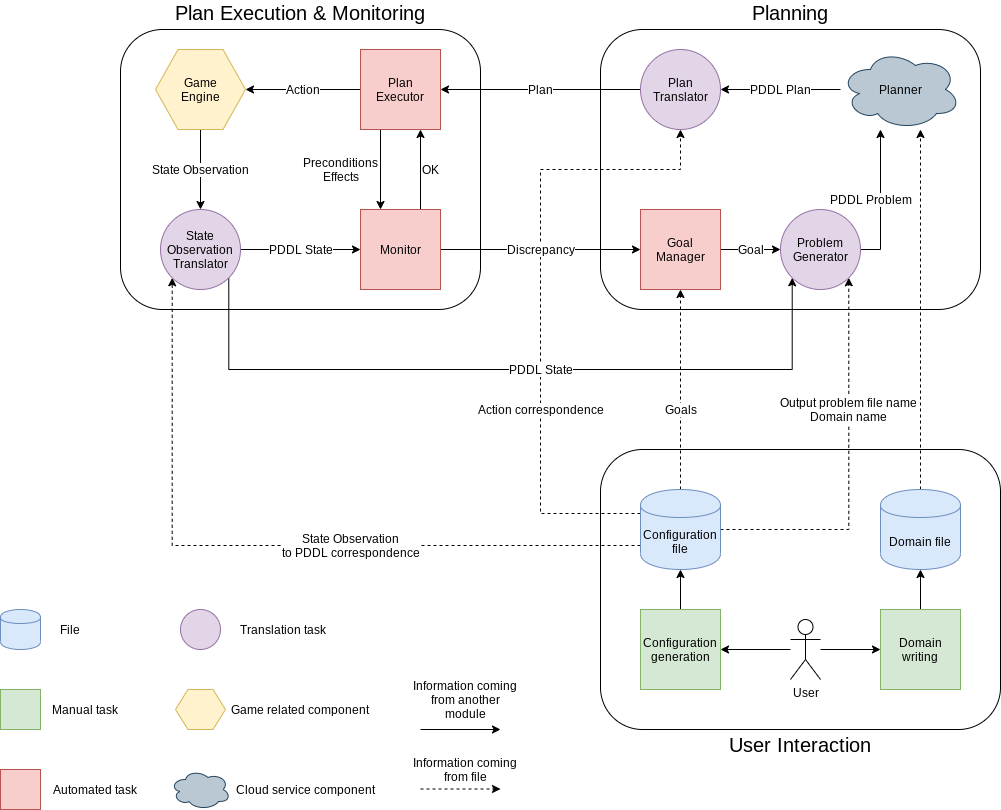
\includegraphics[scale=0.25]{img/presentation/system_arch}
        \end{figure}
    \end{frame}

    %%%%%%%%%%%%%%%%%%%%%%%%%%%%%%%%%%%%%%%%%%%%%%%%%%%%%%%%%%%%%%%%%%%%%%%%%%%%%%%%
    \section{Módulo de interacción con el usuario}

    \begin{frame}{Descripción del módulo}
        \begin{itemize}
            \item Se llevan a cabo dos tareas fundamentales:
                \begin{itemize}
                    \item Creación del \alert{dominio PDDL}.
                    \item Creación del \alert{archivo de configuración}.
                \end{itemize}
            \item No es un componente \textit{software}. Es más bien un \alert{proceso}.
            \item Bajo grado de automatización.
        \end{itemize}
    \end{frame}

    \begin{frame}{Funcionamiento general del módulo}
        \begin{figure}
            \centering
            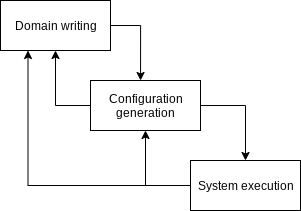
\includegraphics[scale=0.5]{img/presentation/cascade_model}
        \end{figure}
    \end{frame}
    
    \begin{frame}{Creación del dominio}
        \begin{itemize}
            \item Tarea manual llevada a cabo por el usuario.
            \item Utiliza conocimiento:
            \begin{itemize}
                \item Jugar partidas al juego.
                \item Estudiar el archivo VGDL de definición del juego.
            \end{itemize}
        \end{itemize}
    \end{frame}
    
    \begin{frame}{Creación del archivo de configuración}
        \begin{itemize}
            \item Tarea semiautomatizada.
            \item Se dispone de un \textit{script} que genera un archivo de configuración
            plantilla.
            \item Se necesitan el dominio PDDL y el archivo VGDL de definición del juego. 
        \end{itemize}

    \end{frame}
    %%%%%%%%%%%%%%%%%%%%%%%%%%%%%%%%%%%%%%%%%%%%%%%%%%%%%%%%%%%%%%%%%%%%%%%%%%%%%%%%
    \section{Módulo de planificación}

    \begin{frame}{Descripción del módulo}
        \begin{itemize}
            \item Encargado de llevar a cabo todo el proceso de \alert{planificación} y
            \alert{gestión de objetivos}.
            \item Compuesto por los siguientes módulos funcionales:
            \begin{itemize}
                \item Gestor de objetivos
                \item Generador de problemas PDDL
                \item Planificador
                \item Traductor de planes
            \end{itemize}
            \item Funcionamiento automatizado. Necesita dominio PDDL y archivo de configuración
            definidos por el usuario.
        \end{itemize}

    \end{frame}

    \begin{frame}{Funcionamiento general del módulo}
        \begin{figure}
            \centering
            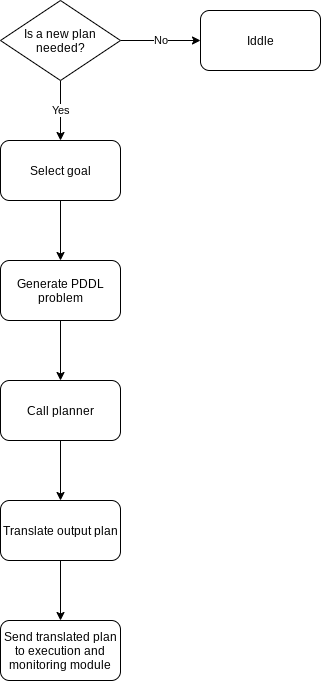
\includegraphics[scale=0.3]{img/presentation/planning_flux}
        \end{figure}
    \end{frame}

    \begin{frame}{Gestor de objetivos}
        \begin{itemize}
            \item Gestionar objetivos y elegir objetivo actual.
            \item Estados de los objetivos:
            \begin{itemize}
                \item \alert{No planificado}
                \item \alert{Alcanzado}
                \item \alert{Detenido}
                \item \alert{Actual}
            \end{itemize}
            \item \alert{Discrepancia}: situación imprevista que se produce en el juego, la
            cual puede \textbf{detener} la ejecución del plan actual o provocar que
            \textbf{un objetivo se alcance prematuramente}.
        \end{itemize}
    \end{frame}

    \begin{frame}{Gestor de objetivos}
        \begin{figure}
            \centering
            \scalebox{0.7}{
                \begin{tikzpicture}
        \node[Node style, state] (not_planned) {Not planned};
        \node[Node style, state, right of=not_planned] (current) {Current goal};
        \node[Node style, state, below of=not_planned] (reached) {Reached};
        \node[Node style, state,right of=reached] (preempted) {Preempted};
        
        \draw (not_planned) edge[above] node{Selected goal} (current)
              (not_planned) edge[left] node{Discrepancy} (reached)
              (current) edge[right, pos=0.2, bend left] node{Discrepancy} (preempted)
              (preempted) edge[left, pos=0.2, bend left] node{Selected goal} (current)
              (preempted) edge[above] node{Discrepancy} (reached)
              (current) edge node[left] {Plan completed} (reached);
\end{tikzpicture}

            }
        \end{figure}
    \end{frame}

    \begin{frame}{Generador de problemas PDDL}
        \begin{itemize}
            \item Genera un problema PDDL hasta el objetivo actual.
            \item \alert{Entradas}
            \begin{itemize}
                \item Objetivo actual
                \item Estado actual del juego en formato PDDL
                \item Nombre del fichero de salida
            \end{itemize}
            \item \alert{Salida}
            \begin{itemize}
                \item Archivo de problema PDDL
            \end{itemize}
        \end{itemize}
    \end{frame}

    \begin{frame}{Planificador}
        \begin{itemize}
            \item Obtiene un plan hasta el objetivo actual.
            \item \alert{Entradas}
            \begin{itemize}
                \item Archivo de dominio PDDL
                \item Archivo de problema PDDL
            \end{itemize}
            \item \alert{Salida}
            \begin{itemize}
                \item Plan hasta el objetivo actual
            \end{itemize}
        \end{itemize}
    \end{frame}

    \begin{frame}{Traductor de planes}
        \begin{itemize}
            \item Traduce los planes obtenidos por el planificador a acciones interpretables
            por el entorno de juegos.
            \item \alert{Entradas}
            \begin{itemize}
                \item Plan hasta el objetivo actual obtenido por el planificador
                \item Correspondencia entre acciones PDDL y acciones GVGAI
            \end{itemize}
            \item \alert{Salida}
            \begin{itemize}
                \item Lista de acciones GVGAI hasta el objetivo actual
            \end{itemize}
        \end{itemize}
    \end{frame}

    %%%%%%%%%%%%%%%%%%%%%%%%%%%%%%%%%%%%%%%%%%%%%%%%%%%%%%%%%%%%%%%%%%%%%%%%%%%%%%%%
    \section{Módulo de ejecución y monitorización}

    \begin{frame}{Descripción del módulo}
        \begin{itemize}
            \item Encargado de \alert{ejecutar} el plan actual y de \alert{supervisar} su ejecución.
            \item Formado por los siguientes módulos funcionales:

            \begin{itemize}
                \item Motor del juego
                \item Traductor del estado de observación
                \item Monitor
                \item Ejecutor del plan
            \end{itemize}
            \item Funcionamiento automatizado. Requiere archivo de configuración definido
            por el usuario.
        \end{itemize}
    \end{frame}

    \begin{frame}{Motor del juego}
        \begin{itemize}
            \item Ejecuta y visualiza el juego.
            \item \alert{Entrada}
            \begin{itemize}
                \item Acción a ejecutar
            \end{itemize}
            \item \alert{Salida}
            \begin{itemize}
                \item Estado de observación actual del juego
            \end{itemize}
        \end{itemize}
    \end{frame}
    
    \begin{frame}{Traductor del estado de observación}
        \begin{itemize}
            \item Traduce el estado de observación del juego a predicados PDDL.
            \item \alert{Entradas}
            \begin{itemize}
                \item Estado de observación del juego
                \item Correspondencia entre los elementos del juego y predicados PDDL
            \end{itemize}
            \item \alert{Salida}
            \begin{itemize}
                \item Estado actual del juego en formato PDDL
            \end{itemize}
        \end{itemize}
    \end{frame}

    \begin{frame}{Monitor}
        \begin{itemize}
            \item Supervisa la ejecución del plan actual.
            \item Estudia la existencia de \alert{discrepancias} en el estado actual del juego.
            \item Se comunica con el \textbf{ejecutor del plan} y el \textbf{gestor de objetivos},
            indicándoles la existencia de discrepancias.
            \item \alert{Entradas}
            \begin{itemize}
                \item Estado actual del juego en formato PDDL
                \item Precondiciones de la acción a ejecutar
                \item Efectos de la acción a ejecutar
            \end{itemize}
        \end{itemize}

    \end{frame}

    \begin{frame}{Funcionamiento del monitor}
        \begin{figure}
            \centering
            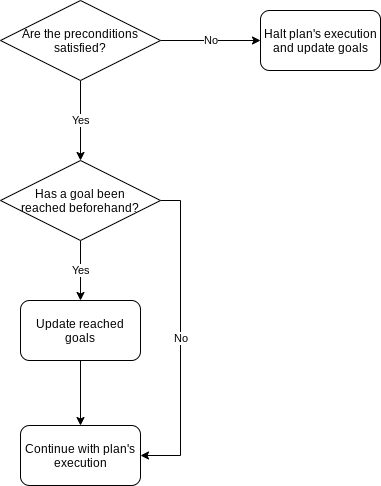
\includegraphics[scale=0.4]{img/presentation/monitor}
        \end{figure}
    \end{frame}

    \begin{frame}{Ejecutor del plan}
        \begin{itemize}
            \item Ejecuta el plan actual.
            \item \alert{Entradas}
            \begin{itemize}
                \item Plan a ejecutar
                \item Señal de control enviada por el monitor indicando si
                el plan actual sigue siendo válido o no
            \end{itemize}
            \item \alert{Salida}
            \begin{itemize}
                \item Siguiente acción a ejecutar del plan actual
            \end{itemize}
        \end{itemize}
    \end{frame}

    %%%%%%%%%%%%%%%%%%%%%%%%%%%%%%%%%%%%%%%%%%%%%%%%%%%%%%%%%%%%%%%%%%%%%%%%%%%%%%%%
    \section{Implementación}

    \begin{frame}{Tecnologías utilizadas}
        \begin{figure}
            \centering
            \begin{subfigure}[t]{0.33\textwidth}
                \centering
                
\includegraphics[scale=1]{img/presentation/java}
            \end{subfigure}%
            \begin{subfigure}[t]{0.33\textwidth}
                \centering
                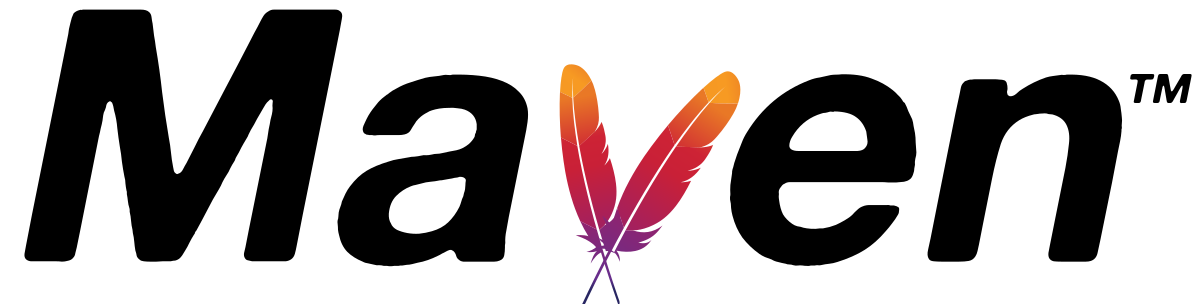
\includegraphics[scale=0.05]{img/presentation/maven}
            \end{subfigure}%
            \begin{subfigure}[t]{0.33\textwidth}
                \centering
                
\includegraphics[scale=0.03]{img/presentation/python}
            \end{subfigure}
            \par\bigskip
            \begin{subfigure}[t]{0.33\textwidth}
                \centering
                
\includegraphics[scale=0.3]{img/presentation/github}
            \end{subfigure}%
            \begin{subfigure}[t]{0.33\textwidth}
                \centering
                
\includegraphics[scale=1]{img/presentation/github-actions}
            \end{subfigure}%
            \begin{subfigure}[t]{0.33\textwidth}
                \centering
                
\includegraphics[scale=0.15]{img/presentation/travisci}
            \end{subfigure}
        \end{figure}
    \end{frame}

    %%%%%%%%%%%%%%%%%%%%%%%%%%%%%%%%%%%%%%%%%%%%%%%%%%%%%%%%%%%%%%%%%%%%%%%%%%%%%%%%
    \section{Experimentación}
    \begin{frame}{Objetivos de la experimentación}
        \begin{itemize}
            \item Se quieren poner a prueba los siguientes aspectos del sistema:
            \begin{enumerate}
                \item Capacidad de generación de problemas PDDL de forma automática.
                \item Capacidad de responder a cambios dinámicos en el entorno durante
                la ejecución del juego.
            \end{enumerate}
        \end{itemize}
    \end{frame}

    \begin{frame}{Juegos utilizados}
        \begin{figure}
            \centering
            \begin{subfigure}[t]{.5\textwidth}
                \centering
                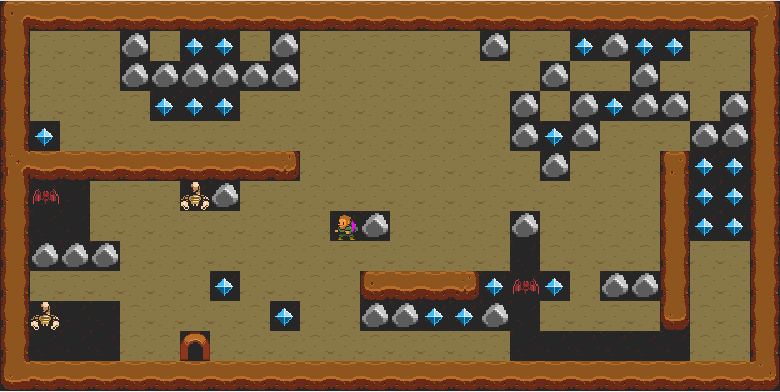
\includegraphics[scale=0.22]{img/presentation/boulderdash.png}
                \caption{\textit{Boulderdash}.}
            \end{subfigure}%
            \begin{subfigure}[t]{.5\textwidth}
                \centering
                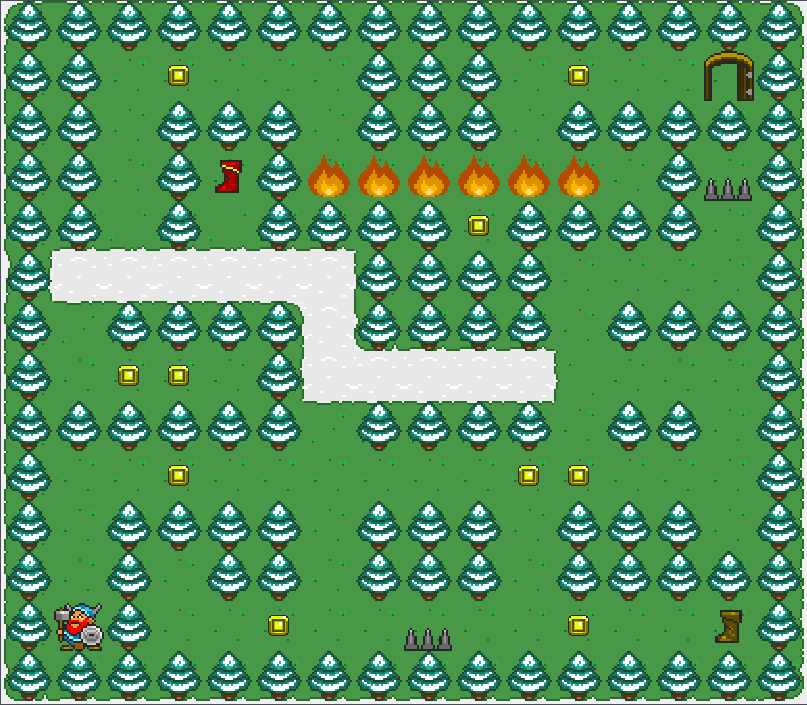
\includegraphics[scale=0.18]{img/presentation/ice_and_fire.png}
                \caption{\textit{Ice and Fire}.}
            \end{subfigure}
            \par\bigskip
            \begin{subfigure}[t]{0.5\textwidth}
                \centering
                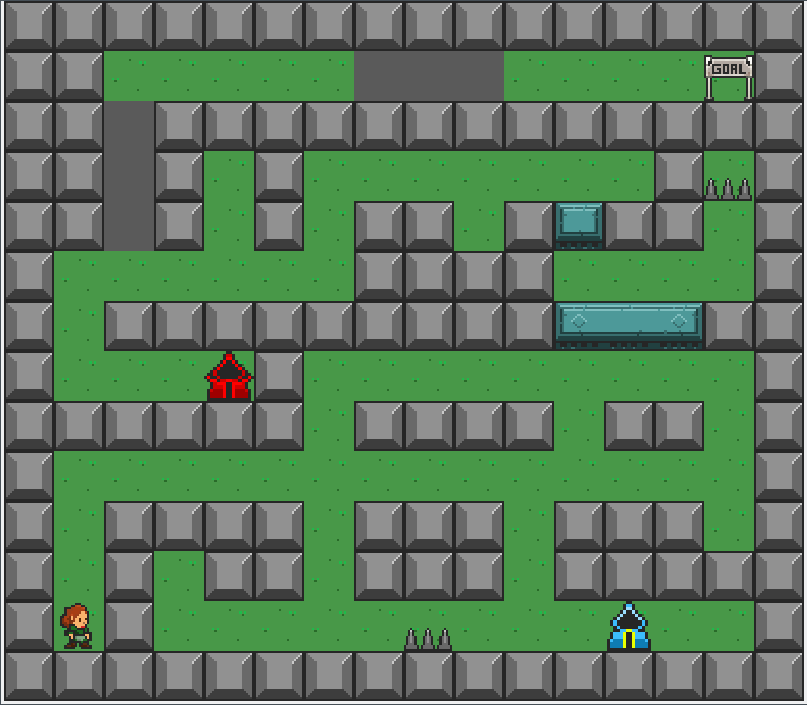
\includegraphics[scale=0.15]{img/presentation/labyrinth_dual.png}
                \caption{\textit{Labyrinth Dual}.}
            \end{subfigure}
        \end{figure}

    \end{frame}

    \begin{frame}{Generación de problemas}
        \begin{table}[]
        \centering
        \resizebox{\textwidth}{!}{%
        \begin{tabular}{|c|c|cccccccc|}
        \hline
        \textbf{Juego} &
          \textbf{Nivel} &
          \textbf{Objetivos} &
          \textbf{\begin{tabular}[c]{@{}c@{}}Predicados problema\\ inicial\end{tabular}} &
          \textbf{\begin{tabular}[c]{@{}c@{}}Objetos problema\\ inicial\end{tabular}} &
          \textbf{\begin{tabular}[c]{@{}c@{}}Tiempo medio\\ ejecución (s)\end{tabular}} &
              \textbf{TPC\footnote{Tiempo de generación de predicados de conectividad} (s)} &
            \textbf{TTEO\footnote{Tiempo de traducción de estados de observación} (s)} &
            \textbf{TGAP\footnote{Tiempo de generación de archivo de problemas} (s)} &
            \textbf{TTGP\footnote{Tiempo total de generación de problema} (s)} \\ \hline
        \multirow{5}{*}{\textit{Boulderdash}}    & \textbf{0} & 10 & \textbf{1735} & \textbf{400} & 0.4967 & 0.0313 & 0.0024 & 0.0038 & \textbf{0.0375} \\ \cline{2-10} 
                                                 & \textbf{1} & 10 & \textbf{1721} & \textbf{393} & 0.428  & 0.0323 & 0.0029 & 0.0039 & \textbf{0.0392} \\ \cline{2-10} 
                                                 & \textbf{2} & 10 & \textbf{1717} & \textbf{391} & 0.5293 & 0.0347 & 0.0034 & 0.0044 & \textbf{0.0425} \\ \cline{2-10} 
                                                 & \textbf{3} & 10 & \textbf{1733} & \textbf{399} & 0.7487 & 0.0327 & 0.0049 & 0.0048 & \textbf{0.0423} \\ \cline{2-10} 
                                                 & \textbf{4} & 10 & \textbf{1731} & \textbf{398} & 0.4403 & 0.0317 & 0.0030 & 0.0039 & \textbf{0.0386} \\ \hline
        \multirow{5}{*}{\textit{Ice and Fire}}   & \textbf{0} & 3  & \textbf{1215} & \textbf{391} & 0.417  & 0.027  & 0.0026 & 0.003  & \textbf{0.0326} \\ \cline{2-10} 
                                                 & \textbf{1} & 3  & \textbf{1234} & \textbf{410} & 0.4827 & 0.0307 & 0.0028 & 0.0056 & \textbf{0.0390} \\ \cline{2-10} 
                                                 & \textbf{2} & 3  & \textbf{1235} & \textbf{411} & 0.522  & 0.0273 & 0.0031 & 0.0045 & \textbf{0.0349} \\ \cline{2-10} 
                                                 & \textbf{3} & 3  & \textbf{1219} & \textbf{395} & 0.4587 & 0.0323 & 0.0029 & 0.0061 & \textbf{0.0413} \\ \cline{2-10} 
                                                 & \textbf{4} & 3  & \textbf{1210} & \textbf{386} & 0.697  & 0.0273 & 0.0031 & 0.0055 & \textbf{0.0359} \\ \hline
        \multirow{5}{*}{\textit{Labyrinth Dual}} & \textbf{0} & 3  & \textbf{1085} & \textbf{369} & 0.4503 & 0.0303 & 0.0029 & 0.0043 & \textbf{0.0376} \\ \cline{2-10} 
                                                 & \textbf{1} & 2  & \textbf{1069} & \textbf{380} & 0.3847 & 0.0303 & 0.0027 & 0.0045 & \textbf{0.0376} \\ \cline{2-10} 
                                                 & \textbf{2} & 3  & \textbf{1073} & \textbf{378} & 0.4107 & 0.0287 & 0.0024 & 0.0029 & \textbf{0,0339} \\ \cline{2-10} 
                                                 & \textbf{3} & 3  & \textbf{1083} & \textbf{376} & 0.41   & 0.0297 & 0.0031 & 0.0052 & \textbf{0.038}  \\ \cline{2-10} 
                                                 & \textbf{4} & 2  & \textbf{1079} & \textbf{363} & 0.5623 & 0.029  & 0.0029 & 0.0062 & \textbf{0.0381} \\ \hline
        \end{tabular}%
        }
        \end{table}
    \end{frame}

    \begin{frame}{Respuesta a cambios dinámicos}
        \begin{figure}
            \centering
            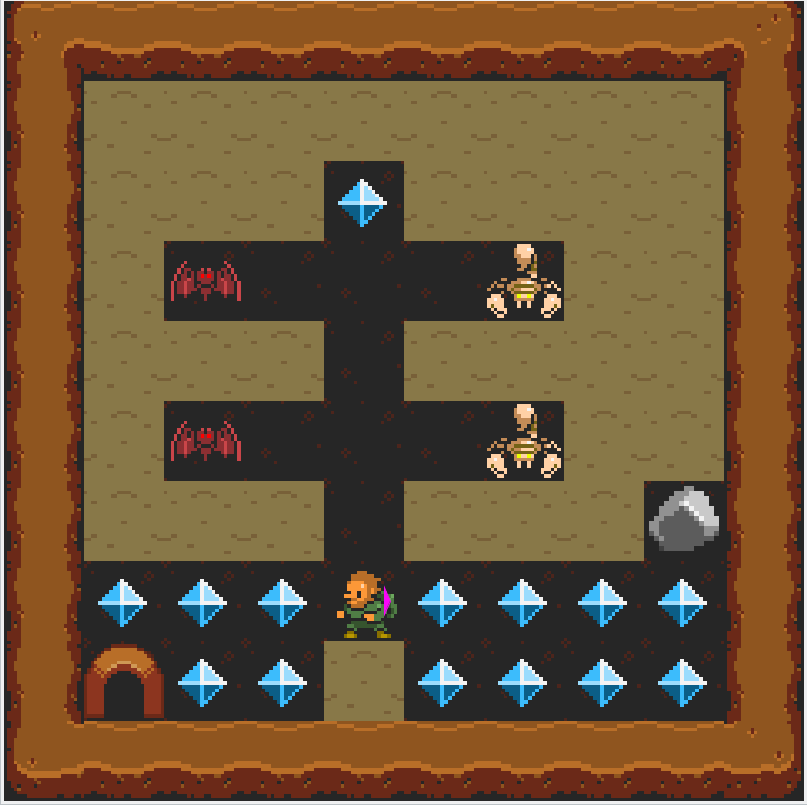
\includegraphics[scale=0.3]{img/presentation/discrepancy}
        \end{figure}
    \end{frame}

    %%%%%%%%%%%%%%%%%%%%%%%%%%%%%%%%%%%%%%%%%%%%%%%%%%%%%%%%%%%%%%%%%%%%%%%%%%%%%%%%
    \section{Conclusiones}

    \begin{frame}{Conclusiones}
        \begin{itemize}
            \item Resolución de múltiples juegos del entorno.
            \item Simplifica y acelera la generación de problemas PDDL.
            \item Herramienta útil para la experimentación con técnicas de planificación
            en GVGAI.
            \item Utilidad para la enseñanza: aprender sobre la planificación y cómo
            generar problemas de planificación.
        \end{itemize}
    \end{frame}

    \begin{frame}{Trabajos futuros}
        \begin{itemize}
            \item Mejora del comportamiento reactivo.
            \item Integración de un módulo de \textit{goal reasoning}.
        \end{itemize}
    \end{frame}

    \begin{frame}[standout]
        \textbf{{\Huge FIN}}
        \noindent\rule[-1ex]{\textwidth}{1.5pt}\\[3.5ex]
        ¿Preguntas?
    \end{frame}
\end{document}
